Das Koaxialkabel wird mit drei unterschiedlichen Abschlussimpedanzen versehen. Alle drei Impedanzen sollen bestimmt werden und je nach der Art der Impedanz die Kapazität~$C$ und Induktivität~$L$ sowie der Widerstand~$R$ bestimmt. Die Eingangsimpedanz ist weiterhin $Z_0 = \SI{50}{\ohm}$.

\subsubsection{Abschlussimpedanz 1}
Der Anzeige des Oszilloskops nach zu urteilen handelt es sich um einen Widerstand und einen Kondensator in Reihenschaltung. Es wird für die aufsteigende Flanke die selbe Fit-Funktion angelegt wie bereits in Kapitel \ref{sec:kapazitat}. Die Messwerte und die Funktion sind in Abb. \ref{fig:box25} dargestellt. Die Parameter sind:
\begin{align}
	a &= \SI{-12.6127}{\volt}
 \\
	b &= \SI{1.1270}{}
 \\
	c &= \SI{0.0017}{\per\farad\per\ohm}
 \\
	d &= \SI{-9.8317}{\nano\second}
 \\
	e &= \SI{1339.6486}{\volt}
 
\end{align}
Daraus ergibt sich für den Widerstand und die Kapazität:
\begin{align}
	R &= \frac{Z_0}{b} - Z_0 = \SI{18.3527}{\ohm}
 \\
	C &= \frac{1}{ c (r + Z_0) \cdot 10^9} = \SI{13241.8832}{\pico\farad}
 \quad.
\end{align}


\begin{figure}
	\centering
	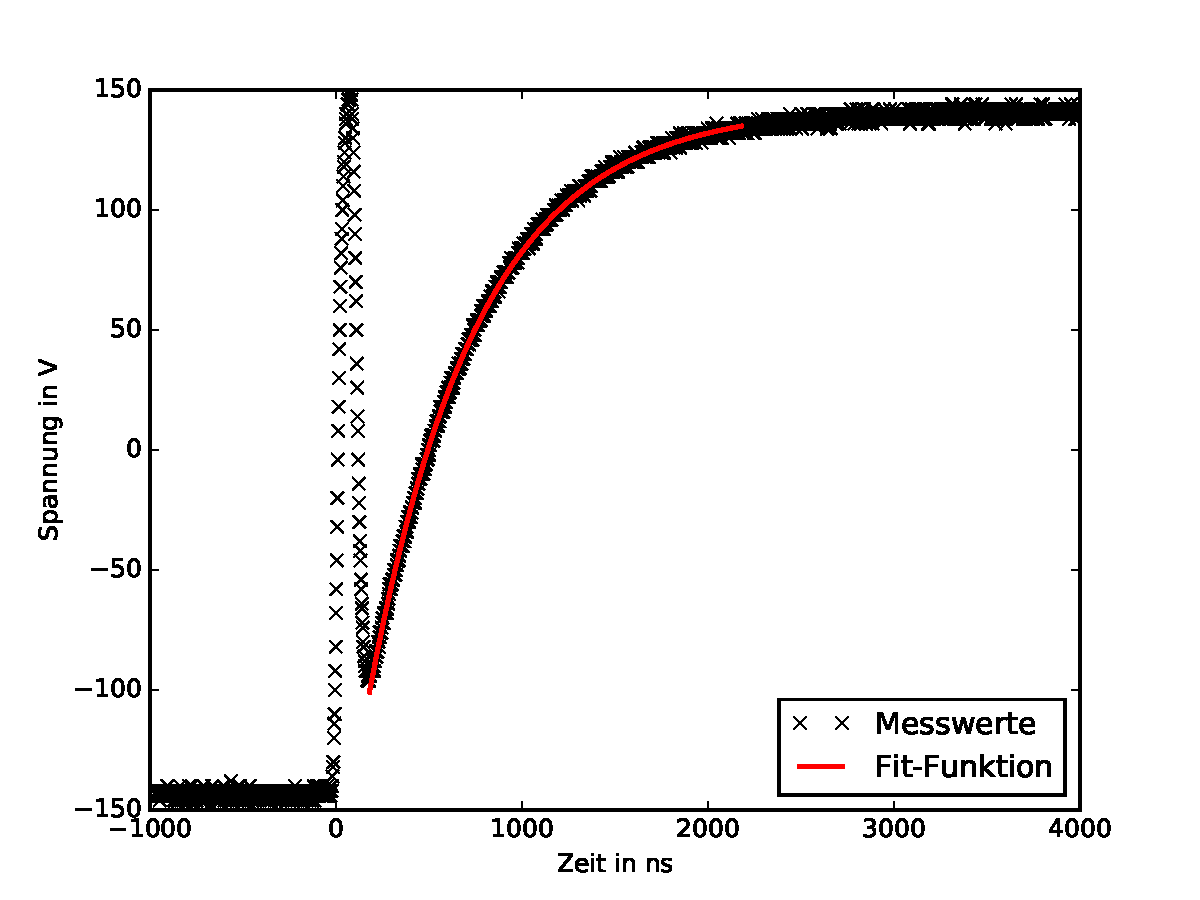
\includegraphics[width=0.7\textwidth]{Box25/Box25.pdf}
	\caption{Spannungsverlauf bei dem Kabel mit Abschlussimpedanz 1}
	\label{fig:box25}
\end{figure}

\subsubsection{Abschlussimpedanz 2}
Bei dieser Abschlussimpedanz handelt es sich um eine Spule und einen Widerstand, die in Reihe geschaltet sind. Die Fit-Funktion ist die selbe wie in Kapitel \ref{sec:impedanz}. Abb. \ref{fig:box23} zeigt die Messwerte ebenso wie die Fit-Funktion. Die Parameter sind:
\begin{align}
	a &= \SI{-12.6127}{\volt}
 \\
	b &= \SI{1.1270}{}
 \\
	c &= \SI{0.0017}{\per\farad\per\ohm}
 \\
	d &= \SI{-9.8317}{\nano\second}
 \\
	e &= \SI{1339.6486}{\volt}
 
\end{align}
Daraus ergibt sich hier für den Widerstand und die Impedanz:
\begin{align}
	R &= \frac{Z_0}{b} - Z_0 = \SI{18.3527}{\ohm}
 \\
	L &= \frac{1}{ c (r + Z_0) \cdot 10^9} = \SI{3.6938}{\micro\henry}
 \quad.
\end{align}

\begin{figure}
	\centering
	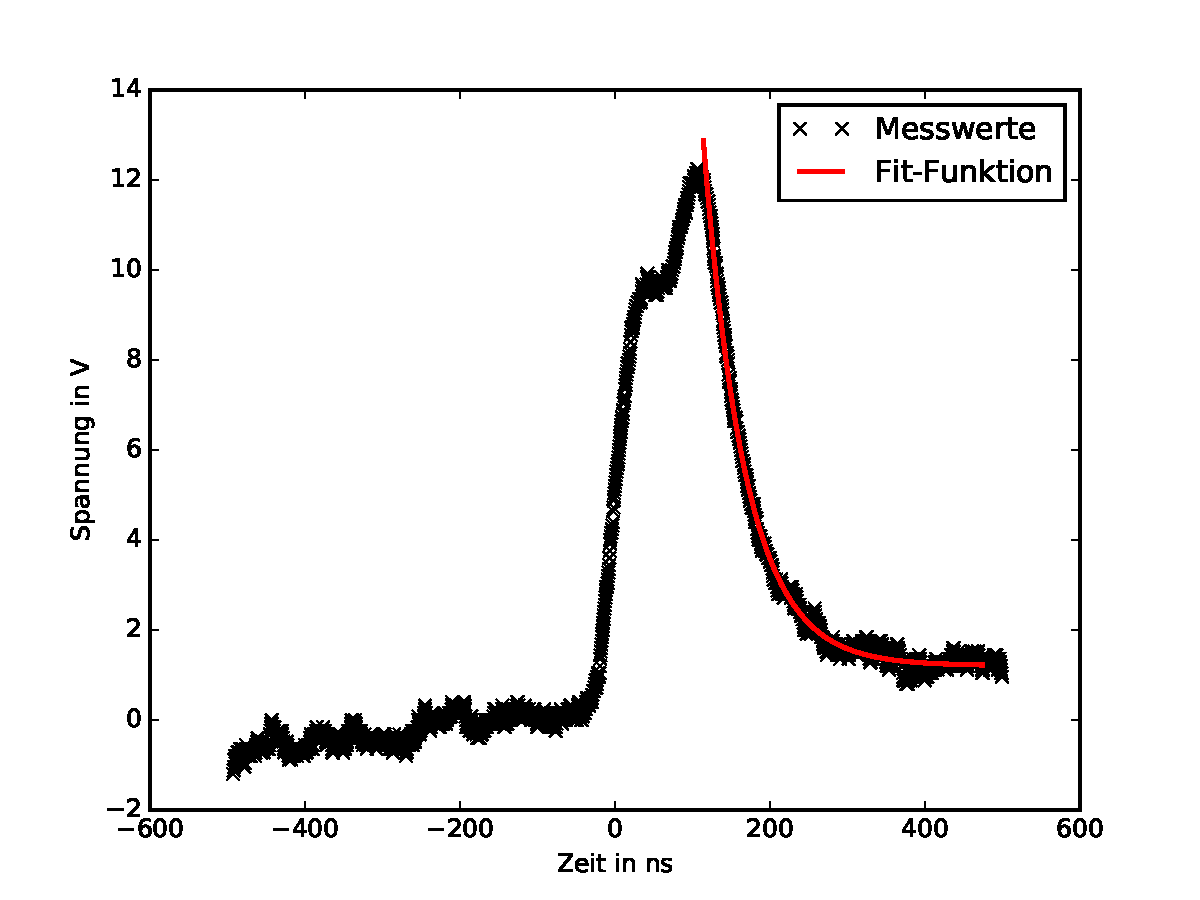
\includegraphics[width=0.7\textwidth]{Box23/Box23.pdf}
	\caption{Spannungsverlauf bei dem Kabel mit Abschlussimpedanz 2}
	\label{fig:box23}
\end{figure}
